% Created by tikzDevice version 0.8.1 on 2015-11-17 11:43:47
% !TEX encoding = UTF-8 Unicode
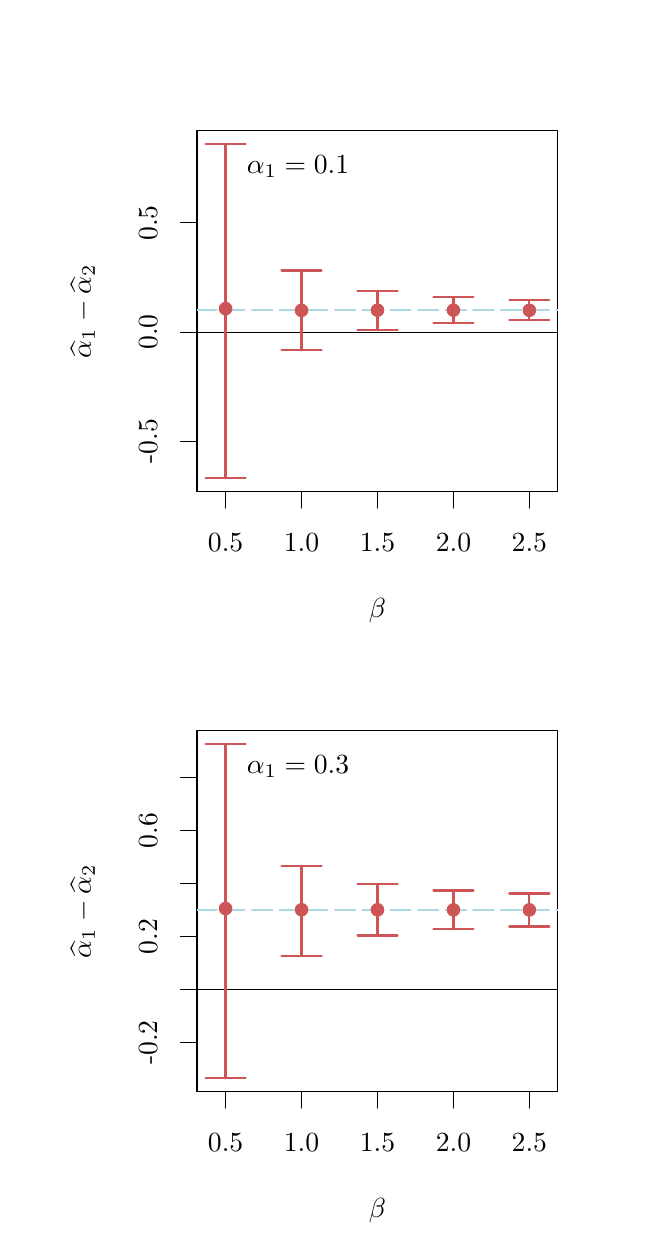
\begin{tikzpicture}[x=1pt,y=1pt]
\definecolor{fillColor}{RGB}{255,255,255}
\path[use as bounding box,fill=fillColor,fill opacity=0.00] (0,0) rectangle (216.81,433.62);
\begin{scope}
\path[clip] ( 61.20,266.01) rectangle (191.61,396.42);
\definecolor{drawColor}{RGB}{255,255,255}
\definecolor{fillColor}{RGB}{255,255,255}

\path[draw=drawColor,line width= 0.4pt,line join=round,line cap=round,fill=fillColor] ( 71.52,332.09) circle (  2.25);

\path[draw=drawColor,line width= 0.4pt,line join=round,line cap=round,fill=fillColor] ( 98.96,331.46) circle (  2.25);

\path[draw=drawColor,line width= 0.4pt,line join=round,line cap=round,fill=fillColor] (126.40,331.52) circle (  2.25);

\path[draw=drawColor,line width= 0.4pt,line join=round,line cap=round,fill=fillColor] (153.85,331.53) circle (  2.25);

\path[draw=drawColor,line width= 0.4pt,line join=round,line cap=round,fill=fillColor] (181.29,331.48) circle (  2.25);
\end{scope}
\begin{scope}
\path[clip] (  0.00,  0.00) rectangle (216.81,433.62);
\definecolor{drawColor}{RGB}{0,0,0}

\path[draw=drawColor,line width= 0.4pt,line join=round,line cap=round] ( 71.52,266.01) -- (181.29,266.01);

\path[draw=drawColor,line width= 0.4pt,line join=round,line cap=round] ( 71.52,266.01) -- ( 71.52,260.01);

\path[draw=drawColor,line width= 0.4pt,line join=round,line cap=round] ( 98.96,266.01) -- ( 98.96,260.01);

\path[draw=drawColor,line width= 0.4pt,line join=round,line cap=round] (126.40,266.01) -- (126.40,260.01);

\path[draw=drawColor,line width= 0.4pt,line join=round,line cap=round] (153.85,266.01) -- (153.85,260.01);

\path[draw=drawColor,line width= 0.4pt,line join=round,line cap=round] (181.29,266.01) -- (181.29,260.01);

\node[text=drawColor,anchor=base,inner sep=0pt, outer sep=0pt, scale=  1.00] at ( 71.52,244.41) {0.5};

\node[text=drawColor,anchor=base,inner sep=0pt, outer sep=0pt, scale=  1.00] at ( 98.96,244.41) {1.0};

\node[text=drawColor,anchor=base,inner sep=0pt, outer sep=0pt, scale=  1.00] at (126.40,244.41) {1.5};

\node[text=drawColor,anchor=base,inner sep=0pt, outer sep=0pt, scale=  1.00] at (153.85,244.41) {2.0};

\node[text=drawColor,anchor=base,inner sep=0pt, outer sep=0pt, scale=  1.00] at (181.29,244.41) {2.5};

\path[draw=drawColor,line width= 0.4pt,line join=round,line cap=round] ( 61.20,284.18) -- ( 61.20,363.07);

\path[draw=drawColor,line width= 0.4pt,line join=round,line cap=round] ( 61.20,284.18) -- ( 55.20,284.18);

\path[draw=drawColor,line width= 0.4pt,line join=round,line cap=round] ( 61.20,323.62) -- ( 55.20,323.62);

\path[draw=drawColor,line width= 0.4pt,line join=round,line cap=round] ( 61.20,363.07) -- ( 55.20,363.07);

\node[text=drawColor,rotate= 90.00,anchor=base,inner sep=0pt, outer sep=0pt, scale=  1.00] at ( 46.80,284.18) {-0.5};

\node[text=drawColor,rotate= 90.00,anchor=base,inner sep=0pt, outer sep=0pt, scale=  1.00] at ( 46.80,323.62) {0.0};

\node[text=drawColor,rotate= 90.00,anchor=base,inner sep=0pt, outer sep=0pt, scale=  1.00] at ( 46.80,363.07) {0.5};

\path[draw=drawColor,line width= 0.4pt,line join=round,line cap=round] ( 61.20,266.01) --
	(191.61,266.01) --
	(191.61,396.42) --
	( 61.20,396.42) --
	( 61.20,266.01);
\end{scope}
\begin{scope}
\path[clip] (  0.00,216.81) rectangle (216.81,433.62);
\definecolor{drawColor}{RGB}{0,0,0}

\node[text=drawColor,anchor=base,inner sep=0pt, outer sep=0pt, scale=  1.00] at (126.41,220.41) {$\beta$};

\node[text=drawColor,rotate= 90.00,anchor=base,inner sep=0pt, outer sep=0pt, scale=  1.00] at ( 22.80,331.22) {$\widehat{\alpha}_1 - \widehat{\alpha}_2$};
\end{scope}
\begin{scope}
\path[clip] ( 61.20,266.01) rectangle (191.61,396.42);
\definecolor{drawColor}{RGB}{0,0,0}

\node[text=drawColor,anchor=base west,inner sep=0pt, outer sep=0pt, scale=  1.00] at ( 79.20,380.98) {$\alpha_1=0.1$};
\definecolor{drawColor}{RGB}{173,216,230}

\path[draw=drawColor,line width= 0.8pt,dash pattern=on 7pt off 3pt ,line join=round,line cap=round] ( 61.20,331.51) -- (191.61,331.51);

\path[draw=drawColor,line width= 0.8pt,dash pattern=on 7pt off 3pt ,line join=round,line cap=round] ( 61.20,331.51) -- (191.61,331.51);

\path[draw=drawColor,line width= 0.8pt,dash pattern=on 7pt off 3pt ,line join=round,line cap=round] ( 61.20,331.51) -- (191.61,331.51);

\path[draw=drawColor,line width= 0.8pt,dash pattern=on 7pt off 3pt ,line join=round,line cap=round] ( 61.20,331.51) -- (191.61,331.51);

\path[draw=drawColor,line width= 0.8pt,dash pattern=on 7pt off 3pt ,line join=round,line cap=round] ( 61.20,331.51) -- (191.61,331.51);
\definecolor{drawColor}{RGB}{0,0,0}

\path[draw=drawColor,line width= 0.4pt,line join=round,line cap=round] ( 61.20,323.62) -- (191.61,323.62);
\definecolor{drawColor}{RGB}{205,85,85}

\path[draw=drawColor,line width= 0.8pt,line join=round,line cap=round] ( 71.52,270.84) -- ( 71.52,391.59);

\path[draw=drawColor,line width= 0.8pt,line join=round,line cap=round] ( 64.29,270.84) --
	( 71.52,270.84) --
	( 78.75,270.84);

\path[draw=drawColor,line width= 0.8pt,line join=round,line cap=round] ( 78.75,391.59) --
	( 71.52,391.59) --
	( 64.29,391.59);

\path[draw=drawColor,line width= 0.8pt,line join=round,line cap=round] ( 98.96,317.03) -- ( 98.96,345.88);

\path[draw=drawColor,line width= 0.8pt,line join=round,line cap=round] ( 91.73,317.03) --
	( 98.96,317.03) --
	(106.19,317.03);

\path[draw=drawColor,line width= 0.8pt,line join=round,line cap=round] (106.19,345.88) --
	( 98.96,345.88) --
	( 91.73,345.88);

\path[draw=drawColor,line width= 0.8pt,line join=round,line cap=round] (126.40,324.38) -- (126.40,338.56);

\path[draw=drawColor,line width= 0.8pt,line join=round,line cap=round] (119.18,324.38) --
	(126.40,324.38) --
	(133.63,324.38);

\path[draw=drawColor,line width= 0.8pt,line join=round,line cap=round] (133.63,338.56) --
	(126.40,338.56) --
	(119.18,338.56);

\path[draw=drawColor,line width= 0.8pt,line join=round,line cap=round] (153.85,326.78) -- (153.85,336.30);

\path[draw=drawColor,line width= 0.8pt,line join=round,line cap=round] (146.62,326.78) --
	(153.85,326.78) --
	(161.08,326.78);

\path[draw=drawColor,line width= 0.8pt,line join=round,line cap=round] (161.08,336.30) --
	(153.85,336.30) --
	(146.62,336.30);

\path[draw=drawColor,line width= 0.8pt,line join=round,line cap=round] (181.29,327.85) -- (181.29,335.20);

\path[draw=drawColor,line width= 0.8pt,line join=round,line cap=round] (174.06,327.85) --
	(181.29,327.85) --
	(188.52,327.85);

\path[draw=drawColor,line width= 0.8pt,line join=round,line cap=round] (188.52,335.20) --
	(181.29,335.20) --
	(174.06,335.20);
\definecolor{fillColor}{RGB}{205,85,85}

\path[draw=drawColor,line width= 0.4pt,line join=round,line cap=round,fill=fillColor] ( 71.52,332.09) circle (  2.25);

\path[draw=drawColor,line width= 0.4pt,line join=round,line cap=round,fill=fillColor] ( 98.96,331.46) circle (  2.25);

\path[draw=drawColor,line width= 0.4pt,line join=round,line cap=round,fill=fillColor] (126.40,331.52) circle (  2.25);

\path[draw=drawColor,line width= 0.4pt,line join=round,line cap=round,fill=fillColor] (153.85,331.53) circle (  2.25);

\path[draw=drawColor,line width= 0.4pt,line join=round,line cap=round,fill=fillColor] (181.29,331.48) circle (  2.25);
\end{scope}
\begin{scope}
\path[clip] ( 61.20, 49.20) rectangle (191.61,179.61);
\definecolor{drawColor}{RGB}{255,255,255}
\definecolor{fillColor}{RGB}{255,255,255}

\path[draw=drawColor,line width= 0.4pt,line join=round,line cap=round,fill=fillColor] ( 71.52,115.33) circle (  2.25);

\path[draw=drawColor,line width= 0.4pt,line join=round,line cap=round,fill=fillColor] ( 98.96,114.88) circle (  2.25);

\path[draw=drawColor,line width= 0.4pt,line join=round,line cap=round,fill=fillColor] (126.40,114.87) circle (  2.25);

\path[draw=drawColor,line width= 0.4pt,line join=round,line cap=round,fill=fillColor] (153.85,114.83) circle (  2.25);

\path[draw=drawColor,line width= 0.4pt,line join=round,line cap=round,fill=fillColor] (181.29,114.84) circle (  2.25);
\end{scope}
\begin{scope}
\path[clip] (  0.00,  0.00) rectangle (216.81,433.62);
\definecolor{drawColor}{RGB}{0,0,0}

\path[draw=drawColor,line width= 0.4pt,line join=round,line cap=round] ( 71.52, 49.20) -- (181.29, 49.20);

\path[draw=drawColor,line width= 0.4pt,line join=round,line cap=round] ( 71.52, 49.20) -- ( 71.52, 43.20);

\path[draw=drawColor,line width= 0.4pt,line join=round,line cap=round] ( 98.96, 49.20) -- ( 98.96, 43.20);

\path[draw=drawColor,line width= 0.4pt,line join=round,line cap=round] (126.40, 49.20) -- (126.40, 43.20);

\path[draw=drawColor,line width= 0.4pt,line join=round,line cap=round] (153.85, 49.20) -- (153.85, 43.20);

\path[draw=drawColor,line width= 0.4pt,line join=round,line cap=round] (181.29, 49.20) -- (181.29, 43.20);

\node[text=drawColor,anchor=base,inner sep=0pt, outer sep=0pt, scale=  1.00] at ( 71.52, 27.60) {0.5};

\node[text=drawColor,anchor=base,inner sep=0pt, outer sep=0pt, scale=  1.00] at ( 98.96, 27.60) {1.0};

\node[text=drawColor,anchor=base,inner sep=0pt, outer sep=0pt, scale=  1.00] at (126.40, 27.60) {1.5};

\node[text=drawColor,anchor=base,inner sep=0pt, outer sep=0pt, scale=  1.00] at (153.85, 27.60) {2.0};

\node[text=drawColor,anchor=base,inner sep=0pt, outer sep=0pt, scale=  1.00] at (181.29, 27.60) {2.5};

\path[draw=drawColor,line width= 0.4pt,line join=round,line cap=round] ( 61.20, 66.91) -- ( 61.20,162.74);

\path[draw=drawColor,line width= 0.4pt,line join=round,line cap=round] ( 61.20, 66.91) -- ( 55.20, 66.91);

\path[draw=drawColor,line width= 0.4pt,line join=round,line cap=round] ( 61.20, 86.08) -- ( 55.20, 86.08);

\path[draw=drawColor,line width= 0.4pt,line join=round,line cap=round] ( 61.20,105.24) -- ( 55.20,105.24);

\path[draw=drawColor,line width= 0.4pt,line join=round,line cap=round] ( 61.20,124.41) -- ( 55.20,124.41);

\path[draw=drawColor,line width= 0.4pt,line join=round,line cap=round] ( 61.20,143.57) -- ( 55.20,143.57);

\path[draw=drawColor,line width= 0.4pt,line join=round,line cap=round] ( 61.20,162.74) -- ( 55.20,162.74);

\node[text=drawColor,rotate= 90.00,anchor=base,inner sep=0pt, outer sep=0pt, scale=  1.00] at ( 46.80, 66.91) {-0.2};

\node[text=drawColor,rotate= 90.00,anchor=base,inner sep=0pt, outer sep=0pt, scale=  1.00] at ( 46.80,105.24) {0.2};

\node[text=drawColor,rotate= 90.00,anchor=base,inner sep=0pt, outer sep=0pt, scale=  1.00] at ( 46.80,143.57) {0.6};

\path[draw=drawColor,line width= 0.4pt,line join=round,line cap=round] ( 61.20, 49.20) --
	(191.61, 49.20) --
	(191.61,179.61) --
	( 61.20,179.61) --
	( 61.20, 49.20);
\end{scope}
\begin{scope}
\path[clip] (  0.00,  0.00) rectangle (216.81,216.81);
\definecolor{drawColor}{RGB}{0,0,0}

\node[text=drawColor,anchor=base,inner sep=0pt, outer sep=0pt, scale=  1.00] at (126.41,  3.60) {$\beta$};

\node[text=drawColor,rotate= 90.00,anchor=base,inner sep=0pt, outer sep=0pt, scale=  1.00] at ( 22.80,114.41) {$\widehat{\alpha}_1 - \widehat{\alpha}_2$};
\end{scope}
\begin{scope}
\path[clip] ( 61.20, 49.20) rectangle (191.61,179.61);
\definecolor{drawColor}{RGB}{0,0,0}

\node[text=drawColor,anchor=base west,inner sep=0pt, outer sep=0pt, scale=  1.00] at ( 79.20,164.17) {$\alpha_1=0.3$};
\definecolor{drawColor}{RGB}{173,216,230}

\path[draw=drawColor,line width= 0.8pt,dash pattern=on 7pt off 3pt ,line join=round,line cap=round] ( 61.20,114.82) -- (191.61,114.82);

\path[draw=drawColor,line width= 0.8pt,dash pattern=on 7pt off 3pt ,line join=round,line cap=round] ( 61.20,114.82) -- (191.61,114.82);

\path[draw=drawColor,line width= 0.8pt,dash pattern=on 7pt off 3pt ,line join=round,line cap=round] ( 61.20,114.82) -- (191.61,114.82);

\path[draw=drawColor,line width= 0.8pt,dash pattern=on 7pt off 3pt ,line join=round,line cap=round] ( 61.20,114.82) -- (191.61,114.82);

\path[draw=drawColor,line width= 0.8pt,dash pattern=on 7pt off 3pt ,line join=round,line cap=round] ( 61.20,114.82) -- (191.61,114.82);
\definecolor{drawColor}{RGB}{0,0,0}

\path[draw=drawColor,line width= 0.4pt,line join=round,line cap=round] ( 61.20, 86.08) -- (191.61, 86.08);
\definecolor{drawColor}{RGB}{205,85,85}

\path[draw=drawColor,line width= 0.8pt,line join=round,line cap=round] ( 71.52, 54.03) -- ( 71.52,174.78);

\path[draw=drawColor,line width= 0.8pt,line join=round,line cap=round] ( 64.29, 54.03) --
	( 71.52, 54.03) --
	( 78.75, 54.03);

\path[draw=drawColor,line width= 0.8pt,line join=round,line cap=round] ( 78.75,174.78) --
	( 71.52,174.78) --
	( 64.29,174.78);

\path[draw=drawColor,line width= 0.8pt,line join=round,line cap=round] ( 98.96, 98.15) -- ( 98.96,130.74);

\path[draw=drawColor,line width= 0.8pt,line join=round,line cap=round] ( 91.73, 98.15) --
	( 98.96, 98.15) --
	(106.19, 98.15);

\path[draw=drawColor,line width= 0.8pt,line join=round,line cap=round] (106.19,130.74) --
	( 98.96,130.74) --
	( 91.73,130.74);

\path[draw=drawColor,line width= 0.8pt,line join=round,line cap=round] (126.40,105.56) -- (126.40,124.15);

\path[draw=drawColor,line width= 0.8pt,line join=round,line cap=round] (119.18,105.56) --
	(126.40,105.56) --
	(133.63,105.56);

\path[draw=drawColor,line width= 0.8pt,line join=round,line cap=round] (133.63,124.15) --
	(126.40,124.15) --
	(119.18,124.15);

\path[draw=drawColor,line width= 0.8pt,line join=round,line cap=round] (153.85,107.85) -- (153.85,121.82);

\path[draw=drawColor,line width= 0.8pt,line join=round,line cap=round] (146.62,107.85) --
	(153.85,107.85) --
	(161.08,107.85);

\path[draw=drawColor,line width= 0.8pt,line join=round,line cap=round] (161.08,121.82) --
	(153.85,121.82) --
	(146.62,121.82);

\path[draw=drawColor,line width= 0.8pt,line join=round,line cap=round] (181.29,108.83) -- (181.29,120.74);

\path[draw=drawColor,line width= 0.8pt,line join=round,line cap=round] (174.06,108.83) --
	(181.29,108.83) --
	(188.52,108.83);

\path[draw=drawColor,line width= 0.8pt,line join=round,line cap=round] (188.52,120.74) --
	(181.29,120.74) --
	(174.06,120.74);
\definecolor{fillColor}{RGB}{205,85,85}

\path[draw=drawColor,line width= 0.4pt,line join=round,line cap=round,fill=fillColor] ( 71.52,115.33) circle (  2.25);

\path[draw=drawColor,line width= 0.4pt,line join=round,line cap=round,fill=fillColor] ( 98.96,114.88) circle (  2.25);

\path[draw=drawColor,line width= 0.4pt,line join=round,line cap=round,fill=fillColor] (126.40,114.87) circle (  2.25);

\path[draw=drawColor,line width= 0.4pt,line join=round,line cap=round,fill=fillColor] (153.85,114.83) circle (  2.25);

\path[draw=drawColor,line width= 0.4pt,line join=round,line cap=round,fill=fillColor] (181.29,114.84) circle (  2.25);
\end{scope}
\end{tikzpicture}
